\documentclass[a4paper]{article}
\usepackage[polish]{babel}
\usepackage{polski}
\usepackage[T1]{fontenc}
\usepackage[utf8]{inputenc}
\usepackage{amsmath}
\usepackage{graphicx,color}
\usepackage{float}
\usepackage{cite}
\usepackage{url}
\usepackage[pdftex,hyperfootnotes=false,pdfborder={0 0 0}]{hyperref}
\usepackage{indentfirst}
\usepackage{subfig}
\usepackage{rotating}
\usepackage{multirow}
\usepackage{listings}
\frenchspacing
%zmiana rozmiarów ramki tekstowej
\addtolength{\hoffset}{-2cm}
\addtolength{\textheight}{4cm}
\addtolength{\textwidth}{4cm}
\addtolength{\voffset}{-2cm}
%Sprawdzanie pisowni: aspell -t -l pl -c sprawozdanie.tex

\begin{document}
\thispagestyle{empty}
\begin{center}
{\LARGE{Tartak\\}}
\vspace{3ex}
\begin{tabular}{llr}
\textbf{Łukasz Wieczorek} & inf94385 & wieczorek1990@gmail.com\\
\end{tabular}
\end{center}
\section{Dane}
\begin{itemize}
\item Roczny obrót: 12 milionów,
\item Roczny zysk: 100 tysięcy,
\item Koszt audytu 20 tysięcy,
\item Kwota kredytu, za który kupujemy tartak: 1 milion,
\item Kredyt bierzemy na 5 lat,
\item Oprocentowanie kredytu: 8\%,
\item Podział kosztów: 50\% wynagrodzenia, 50\% materiały,
\item Koszt wynagrodzenia zarządcy po przejęciu tartaku: 50 tysięcy rocznie,
\item Popyt rośnie od 0\% do 80\%, 20\% rocznie (5 lat),
\item Wykorzystanie maszyn 50\%,
\item 50 pracowników, w tym 10 administratorów,
\item Każdy wózek ciągną 2 osoby,
\item Obciążenie magazynów 80\%,
\item Magazyn starcza na 1 miesiąc działalności,
\item Firma nie ma kredytów,
\item Zyski ze sprzedaży: 80\% deski, 18\% belki, 2\% reszta,
\item Czas transportu pomiędzy maszynami nie przekracza 10\% czasu wykonania na maszynach.
\item Liczba maszyn: 3 korujące, 1 tnąca na belki, 2 tnące na deski,
\item Proces produkcji wygląda następująco:
\begin{figure}[H]
\centering
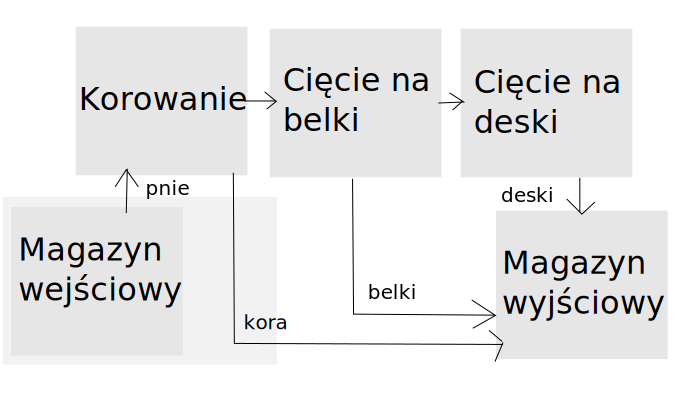
\includegraphics[scale=0.5]{img/Tartak.pdf}
\end{figure}
\end{itemize}
\section{Analiza dochodowości}
Na podstawie założenia, że popyt będzie rocznie rósł wykonałem analizę dochodowości. Analiza zakłada, że koszty pracownicze pozostaną na stałym poziomie. Z analizy (Tablica \ref{tab:1}) wynika, że firma w ciągu 5 lat zarobi około 10,93 miliona zł, jeżeli nadąży z produkcją.
\begin{sidewaystable}
\centering
\begin{tabular}{|l|l|l|l|l|l|}
\hline
Rok  & Popyt        & Obrót              & Koszty odsetek kredytu & Koszty spłaty kredytu & Koszt zarządcy \\ \hline
1    & 100,00\%     & 12000000           & 80000                  & 0                     & 50000          \\ \hline
2    & 120,00\%     & 14400000           & 80000                  & 0                     & 50000          \\ \hline
3    & 140,00\%     & 16800000           & 80000                  & 0                     & 50000          \\ \hline
4    & 160,00\%     & 19200000           & 80000                  & 0                     & 50000          \\ \hline
5    & 180,00\%     & 21600000           & 80000                  & 1000000               & 50000          \\ \hline
SUMA &              & 84000000           & 400000                 & 1000000               & 250000         \\ \hline
Rok  & Koszt audytu & Koszty pracownicze & Koszty materiału       & Koszty całkowite      & Zysk           \\ \hline
1    & 20000        & 5950000            & 5950000                & 12050000              & -50000         \\ \hline
2    & 0            & 5950000            & 7140000                & 13220000              & 1180000        \\ \hline
3    & 0            & 5950000            & 8330000                & 14410000              & 2390000        \\ \hline
4    & 0            & 5950000            & 9520000                & 15600000              & 3600000        \\ \hline
5    & 0            & 5950000            & 10710000               & 17790000              & 3810000        \\ \hline
SUMA & 20000        & 29750000           & 41650000               & 73070000              & 10930000       \\ \hline
\end{tabular}
\caption{Wyniki}
\label{tab:1}
\end{sidewaystable}
\section{Analiza poprawy dochodowości}
Co można zrobić, aby firma była bardziej dochodowa:
\begin{itemize}
\item Wymienić wózki na taśmę produkcyjną,
\item Wprowadzić pracę na więcej zmian,
\item Rozbudować magazyn,
\item Zwiększyć wykorzystanie maszyn (np. system powiadamiania o dostępności maszyn, predykcja zakończenia przetwarzania na maszynach w celu szybszego transportu),
\item Zmniejszyć wynagrodzenia,
\item Wprowadzić bufory przy maszynach,
\item Dokupić maszyny.
\end{itemize}
\section{Symulacja TBS}
Wykonałem symulacje na podstawie poniższego modelu w oprogramowaniu Tibco Business Studio(\cite{tibco:000}).
\begin{figure}[H]
\centering
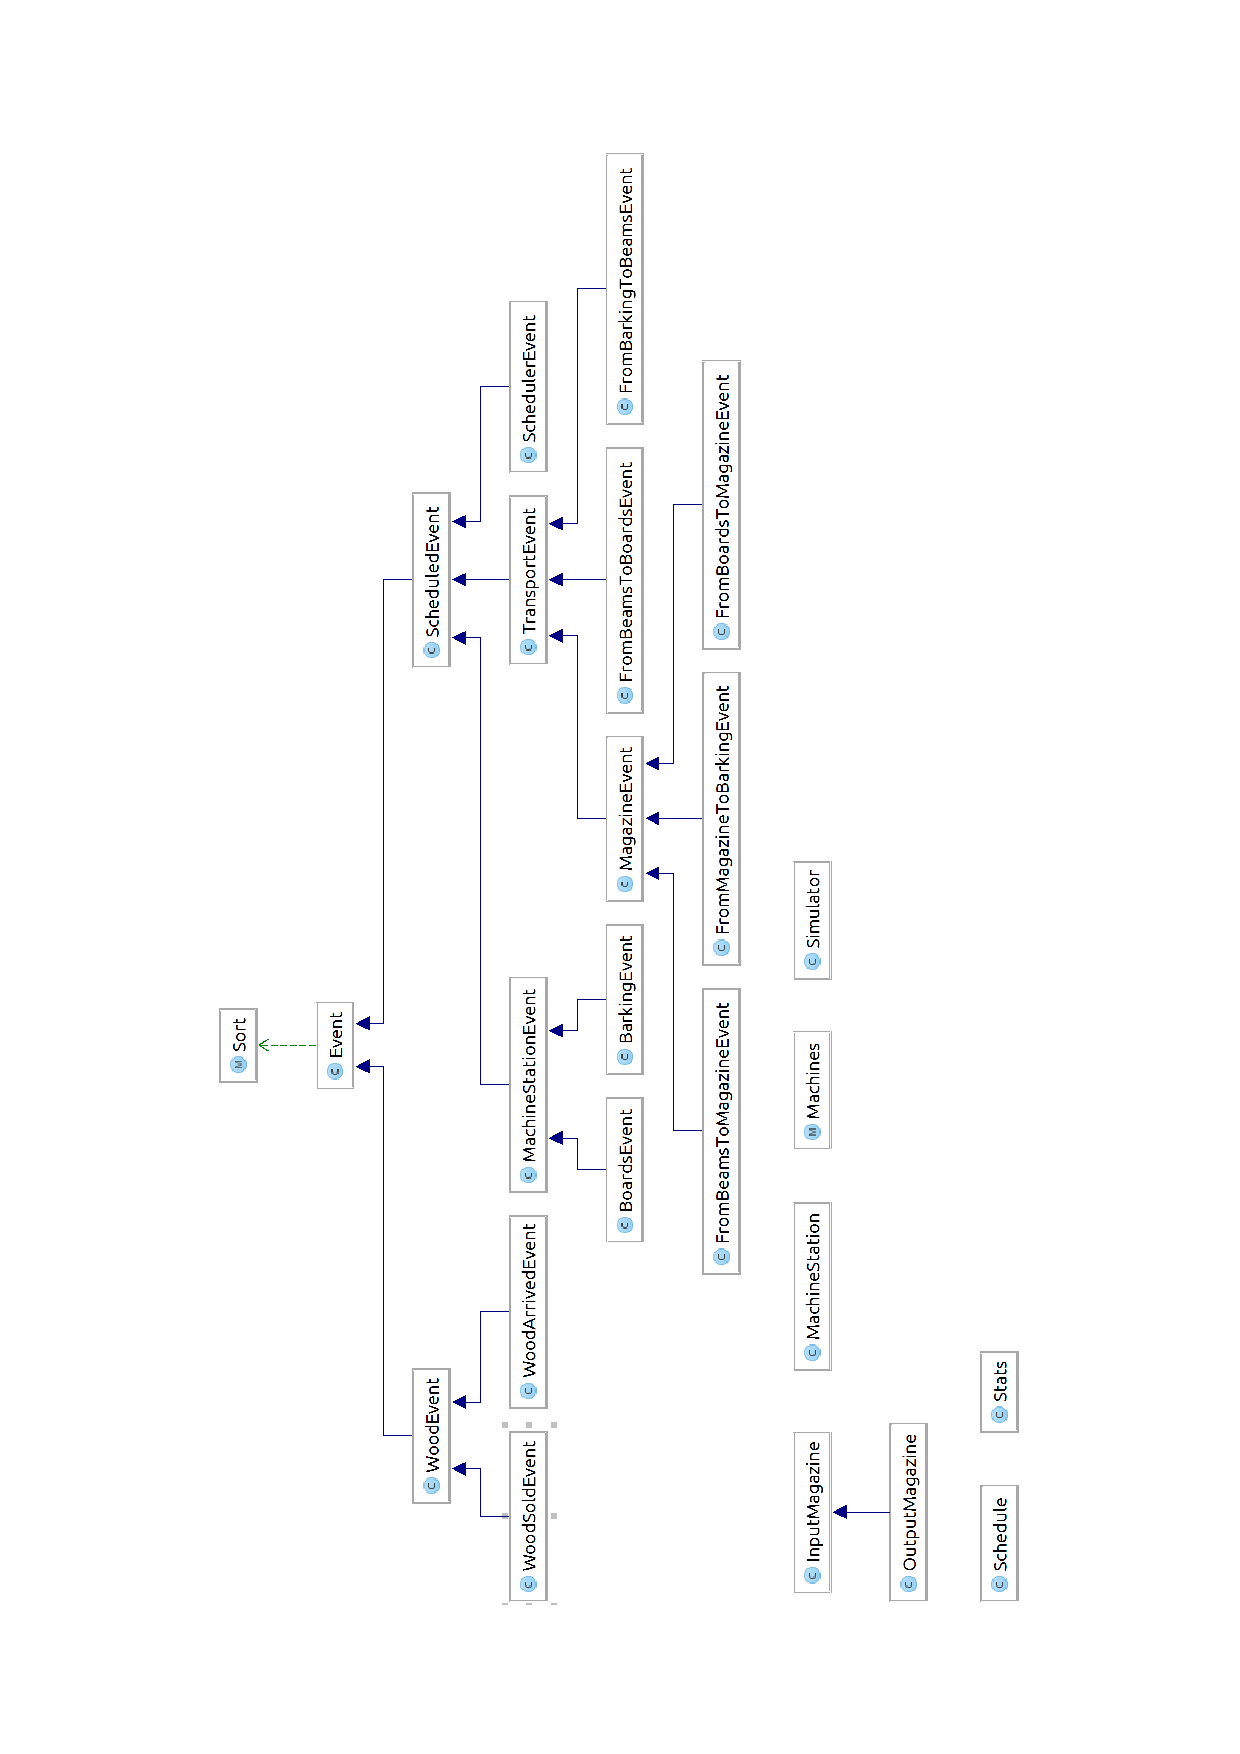
\includegraphics[scale=0.5]{img/diagram.png}
\caption{Model BPMN tartaku}
\label{img:diag}
\end{figure}
Symulacje nazwałem odpowiednio:
\begin{enumerate}
\item 10 wózkowych -- w tartaku jest 10 wózkowych
\item taśma zamiast wózkowych -- 10 wózkowych zastępują taśmy produkcyjne
\end{enumerate}
Założyłem, w ciągu 8-godzinnego dnia pracy przychodzą 4 zleceń obróbki drewna średnio co 60 minut, co daje czasy przetwarzania rzędu 440 minut -- prawie 8 godzin pracy. Z danych zadania wyliczyłem średnią płacę godzinową 59,5 zł (śmiech). Ponadto wykorzystałem następujące dane wejściowe do symulacji:
\begin{table}[H]
\centering
\begin{tabular}{|l|l|l|l|l|l|}
\hline
\multicolumn{6}{|c|}{Pracownicy}                                                        \\ \hline
Wersja             & Pracowników     & Wózkowych & Korowanie & Cięcie & Cięcie na deski \\ \hline
1                  & 40              & 10        & 15        & 5      & 10              \\ \hline
2                  & 40              & 0         & 15        & 5      & 10              \\ \hline
\multicolumn{6}{|c|}{Czasy}                                                             \\ \hline
Wersja             &                 & Przewóz   & Korowanie & Cięcie & Cięcie na deski \\ \hline
\multirow{2}{*}{1} & Średnia         & 3         & 90        & 30     & 60              \\ \cline{2-6} 
                   & Odchylenie std. & 1         & 30        & 10     & 20              \\ \hline
\multirow{2}{*}{2} & Średnia         & 1         & 90        & 30     & 60              \\ \cline{2-6} 
                   & Odchylenie std. & 1         & 30        & 10     & 20              \\ \hline
\end{tabular}
\caption{Dane wejściowe do symulacji}
\label{tab:2}
\end{table}
\subsection{Porównanie}
Porównanie dotyczy zamiany 10 wózkowych na taśmę produkcyjną.
\begin{figure}[H]
\centering
\includegraphics[scale=0.3]{img/case-times.png}
\label{img:cost}
\caption{Średnie czasy cyklu}
\end{figure}
\begin{figure}[H]
\centering
\includegraphics[scale=0.3]{img/case-cost.png}
\label{img:cost}
\caption{Średnie koszty cyklu}
\end{figure}
\subsubsection{Wnioski}
Średni czas cyklu zmniejszył się o 6\%, a średni koszt cyklu zmniejszył się o 9\%. Warto wymienić wózkowych na taśmę produkcyjną. Jakkolwiek zmniejszenie czasu cyklu jest logiczne, to zmniejszenie kosztów o 9\% wydaje się absurdalne, ponieważ zwolniliśmy 10 z 50 pracowników co powinno przełożyć się na 20\% procentową obniżkę kosztów. Powyższe ilustruje, że oprogramowanie TBS w dziwny sposób oblicza koszty. Z tego też powodu zdecydowałem się zbudować własny symulator tartaku.
\section{Symulator}
\subsection{Założenia}
\begin{itemize}
\item Symulacja nie bierze pod uwagę zysków z kory,
\item Symulacja nie bierze pod uwagę kosztów pracowniczych,
\item 81,633\% belek przechodzi proces cięcia na deski,
\end{itemize}
\subsection{Opis danych wejściowych}
\begin{itemize}
\item $simulation\_duration$ -- czas trwania symulacji w minutach,
\item $boards\_percentage$ -- procent drewna przerabianego na deski,
\item $parallel\_carts$ -- liczba mogących równolegle jechać wózków,
\item $wood\_batch$ -- ilość drzewa jaką przewozi jeden wózek, jaka jest przetwarzana w maszynach,
\item $boards\_from\_beam$ -- liczba desek z belki,
\item $barking\_machines$ -- liczba maszyn korujących,
\item $beams\_machines$ -- liczba maszyn tnących na belki,
\item $boards\_machines$ -- liczba maszyn tnących na deski,
\item $wood\_price$ -- cena zakupu pnia,
\item $beam\_price$ -- cena belki,
\item $board\_price$ -- cena deski,
\item $barking\_duration$ -- czas trwania korowania w minutach,
\item $beams\_duration$ -- czas trwania cięcia na belki w minutach,
\item $boards\_duration$ -- czas trwania cięcia na deski w minutach,
\item $input\_magazine\_starting\_capacity$ -- początkowe zapełnienie magazynu wejściowego w liczbie pni,
\item $input\_magazine\_maximal\_capacity$ -- maksymalna pojemność magazynu wejściowego w liczbie pni,
\item $output\_magazine\_starting\_capacity$ -- początkowe zapełnienie magazynu wyjściowego w liczbie belek (deski są traktowane jako części belki),
\item $output\_magazine\_maximal\_capacity$ -- maksymalna pojemność magazynu wyjściowego w liczbie belek (j.w.),
\item $output\_magazine\_beams$ -- liczba belek znajdujących się w magazynie wyjściowym,
\item $output\_magazine\_boards$ -- liczba desek znajdujących się w magazynie wyjściowym,
\item $wood\_arrived\_count$ -- liczba pni przychodzących w wydarzeniu napełniania magazynu,
\item $wood\_sold\_count$ -- liczba belek sprzedawanych w wydarzeniu sprzedaży,
\item $wood\_arrival\_cycle\_time$ -- czas cyklu zdarzenia napełniania magazynu,
\item $wood\_selling\_cycle\_time$ -- czas cyklu zdarzenia sprzedaży,
\item $magazine\_barking\_transport\_duration$ -- czas transportu z magazynu wejściowego do korowania,
\item $barking\_beams\_transport\_duration$ -- czas transportu z korowania do cięcia na belki,
\item $beams\_boards\_transport\_duration$ -- czas transportu z cięcia na deski do cięcia na belki,
\item $boards\_magazine\_transport\_duration$ -- czas transportu z cięcia na deski do magazynu wyjściowego,
\item $beams\_magazine\_transport\_duration$ -- czas transportu z cięcia na belki do magazynu wyjściowego.
\end{itemize}
\subsection{Przykładowa instancja}
\subsubsection{Dane wejściowe}
\lstinputlisting{lst/small.yml}
\subsubsection{Wynik działania}
\lstinputlisting{lst/small.txt}
\subsection{Potrzebne dane}
W celu przeprowadzenia symulacji potrzebowałem różnych danych, przedstawia je poniższy arkusz:
\begin{figure}[H]
\centering
\includegraphics[scale=0.5]{img/arkusz.png}
\caption{Potrzebne dane. Żółte pola to zmienne.}
\end{figure}
\subsection{Założenie o 50\% wykorzystaniu maszyn}
50\% procentowe wykorzystanie maszyn udało mi się uzyskać dla instancji, w której czasy przewozu drewna pomiędzy maszynami i magazynami były bardzo długie, tj. 300 minut.
Średnie wykorzystanie maszyn dla badanych instancji wynosiło ok. 94\% dla liczby maszyn (3, 1, 2), ok. 83,5\% dla (4, 2, 3), ok. 85.5\% dla (5, 2, 4).
\subsection{Analiza wzrostu popytu}
\subsubsection{Dane wejściowe symulacji}
\lstinputlisting{lst/year0.yml}
\subsubsection{Zmiany konieczne do zaspokojenia popytu}
\begin{itemize}
\item W trzecim roku zakup po jednej maszynie każdego rodzaju,
\item W piątym roku zakup maszyny do korowania i do cięcia na deski, rozbudowa magazynu wyjściowego (podwójna pojemność), zwiększenie rozmiaru dostaw drewna z 50 do 75.
\end{itemize}
\section{Wnioski}
50\% wykorzystanie maszyn, co pokazuje symulacja, można zwiększyć do około 80-95\% poprzez lepsze zarządzanie procesem produkcyjnym. Jeśli założyć, że popyt będzie rosnąć według danych, to opłaca się kupić tartak. Natomiast chęć zaspokojenia całego popytu wiąże się z koniecznością rozbudowania magazynów i dokupowania maszyn, dlatego też wydaje się, iż opłaca się dokupić tylko po jednej maszynie każdego rodzaju na początku roku trzeciego, chyba że popyt miałby w przyszłych latach dalej rosnąć.
\bibliography{bibliografia}{}
\bibliographystyle{IEEEtran}
\end{document} 